%----------------------------------------------------------------------------------------
%	Resonance circuit
%----------------------------------------------------------------------------------------
\newcommand*{\resonanceCircuit}{\begingroup
\clearpage
\section{Resonanzkreis}\label{sec:resonancecircuit}
{\noindent

\begin{wrapfigure}{r}{0.5\textwidth}
    \begin{minipage}[r]{0.5\textwidth}
      \vspace{-16pt}
    \begin{figure}[H]
      \centering
      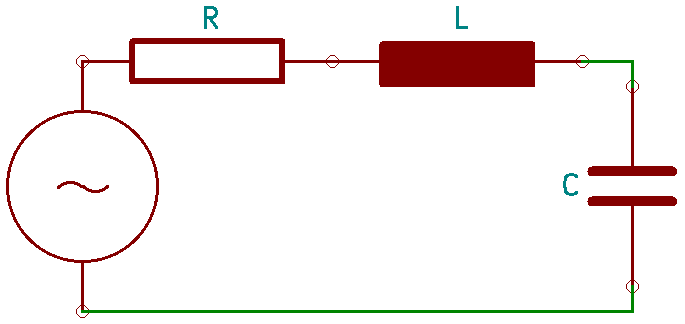
\includegraphics[width=\textwidth]{Graphics/ResonanceCircuit_serial.png}
      \caption{Reihenresonanzkreis}{}
      \label{resonance_circuit_serial_1}
    \end{figure}
    \begin{figure}[H]
      \centering
      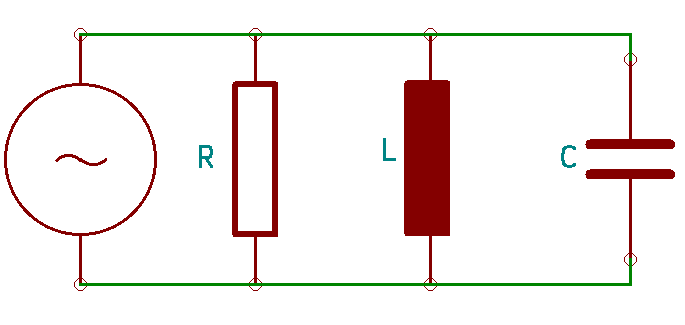
\includegraphics[width=\textwidth]{Graphics/ResonanceCircuit_parallel.png}
      \caption{Parallelresonanzkreis}{}
      \label{resonance_circuit_parallel}
    \end{figure}
    \vspace{-10pt}  
    \end{minipage}  
\end{wrapfigure}

\noindent Resonanzkreise lassen sich generell in Reihenresonanzkreise (Abbildung \ref{resonance_circuit_serial_1}) und Parallelresonanzkreise (Abbildung \ref{resonance_circuit_parallel}) einteilen. Parallelresonanzkreise weisen die Eigenschaft auf, dass die Spannung an allen Stellen der Schaltung gleich und der Strom jeweils abhängig von den Bauelementen an der Messstelle ist. In einem Reihenresonanzkreis hingegen fließt an allen Stellen der gleiche Strom. Die Spannung an den Bauelementen variiert abhängig von der Dimensionierung jener. Diese Eigenschaften machen den Parallelresonanzkreis an dieser Stelle uninteressant. Deshalb wird dieser in diesem Dokument nicht weiter Thematisiert. Im Folgendem ist mit einem Resonanzkreis also immer ein Reihenresonanzkreis gemeint. Ein Resonanzkreis ist, wie der Name vermuten lässt, ein schwingfähiges System. Um zu verstehen wie diese Schwingungen zustande kommen, ist es sinnvoll sich zunächst einmal mit den beiden wichtigsten Bauelementen eines Resonsnzkreises, nämlich dem Kondensator \textbf{C} und der Spule \textbf{L}, zu befassen\footnote{Hagmann, Gerd: Grundlagen der Elektrotechnik. 16. Auflage: AULA-Verlag GmbH, S. 296 ff.}.
\clearpage
\capacitor
\coil
\serialResonanceCircuit

}
\endgroup}
%----------------------------------------------------------------------------------------

%----------------------------------------------------------------------------------------
%	Capacitor
%----------------------------------------------------------------------------------------
\newcommand*{\capacitor}{\begingroup
\subsection{Kondensator}\label{sec:capacitor}
{\noindent Wird ein Kondensator, wie in Abbildung \ref{charge_capacitor_circ} dargestellt, durch eine Betriebsspannung \textbf{U} geladen, 

\begin{wrapfigure}{r}{0.5\textwidth}
    \begin{minipage}[r]{0.5\textwidth}
      \vspace{-16pt}
        \begin{figure}[H]
          \centering
          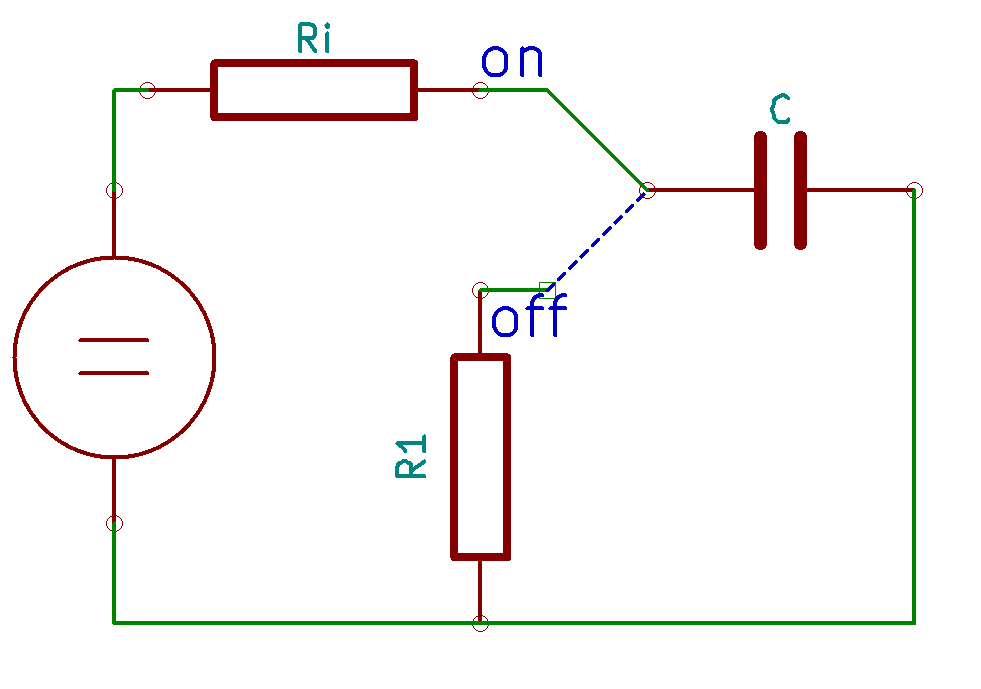
\includegraphics[width=\textwidth]{Graphics/RC_circuit_charge.png}    
          \caption{RC-Schaltung, Kondensator laden}{}
          \label{charge_capacitor_circ}
        \end{figure}
      \vspace{-10pt}  
    \end{minipage}  
\end{wrapfigure}

\noindent so ergibt sich ein Ladestrom von

\begin{equation}
  I_c = \frac{U-U_c}{R_i}
  \label{eq:capacitorCurrent}
\end{equation}

\noindent \(R_i\) stellt hierbei den Innenwiderstand der Spannungsquelle dar und begrenzt den maximalen Ladestrom \(I_c\). Während des Ladevorgangs gleicht sich \(U_c\) der Betriebsspannung \textbf{U} an. Bezogen auf die Gleichung \eqref{eq:capacitorCurrent} bedeutet dies, dass der Ladestrom \(I_c\) bei \(U_c = 0\) seinen Maximum hat und mit Angleichen von \(U_c\) an \textbf{U} kontinuierlich kleiner wird. Es besteht also eine zeitliche Verzögerung zwischen \(I_{cMax}\) und \(u_{cMax}\). Man sagt auch \textbf{am Kondensator eilt der Strom der Spannung voraus!} Die Zeit, die ein Kondensator benötigt, bis \(U_c \approx U\) ist, ist abhängig von der Kapazität \textbf{C} des Kondensators und dem Widerstand \(R_i\). Rechnerisch darstellen lässt sich der zeitliche Verlauf über die Zeitkonstante \(\tau\) nach folgender Gleichung.

\begin{equation}
  \tau_c = R_i \cdot C
  \label{eq:tauCapacitor}
\end{equation}

\noindent Generell gilt, dass ein anfangs komplett entladener Kondensator nach Ablauf eines \(\tau \) auf 63\% der Betriebsspannung \textbf{U} geladen und der Ladestrom \(I_c\) auf 37\% von \(I_{cMax}\) abgefallen ist. Nach Ablauf eines weiteren \(\tau \) ist \(U_c\) nochmals um 63\% der Differenz zwischen \textbf{U} und \(U_c\) angestiegen und \(I_c\) auf 37\% des letzten \(I_c\) abgefallen. Dies führt sich mit jedem Ablauf weiterer \(\tau \) fort, sodass erkennbar wird, dass ein Ladestatus von 100\% nie erreicht wird. Nach Ablauf von \(5\tau \) gilt ein Kondensator mit 99,3\% praktisch als voll aufgeladen und es ergibt sich eine Ladekurve nach dem wie auf Abbildung \ref{charge_capacitor} dargestellten Beispiel. 

\clearpage

%\begin{wrapfigure}{r}{0.75\textwidth}
    %\begin{minipage}[r]{0.75\textwidth}
      %\vspace{-16pt}
      \begin{figure}[H]
        \centering
        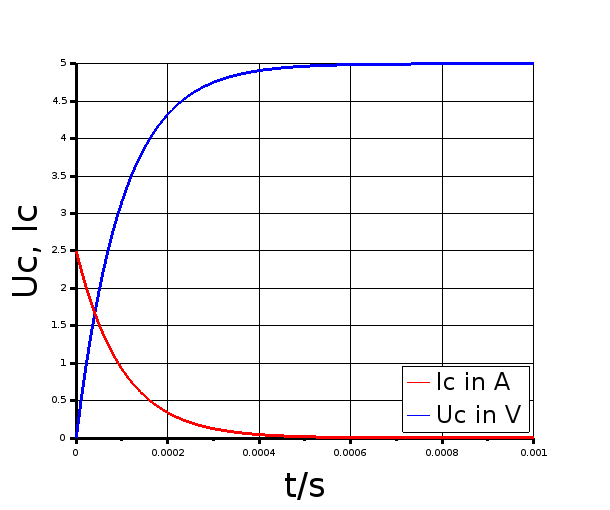
\includegraphics[width=\textwidth]{Graphics/KondensatorLadekurve.png}
        \caption{R=2Ohm, C=50µF, Kondensator laden}{}
        \label{charge_capacitor}
      \end{figure}
      %\vspace{-10pt}  
    %\end{minipage}  
%\end{wrapfigure}
\noindent Wird ein vollständig geladener Kondensator über einen Widerstand \(R_1\) entladen (Abbildung \ref{discharge_capacitor_circ}), so ändert sich die Richtung des Stroms \(I_c\).

\begin{figure}[H]
  \centering
      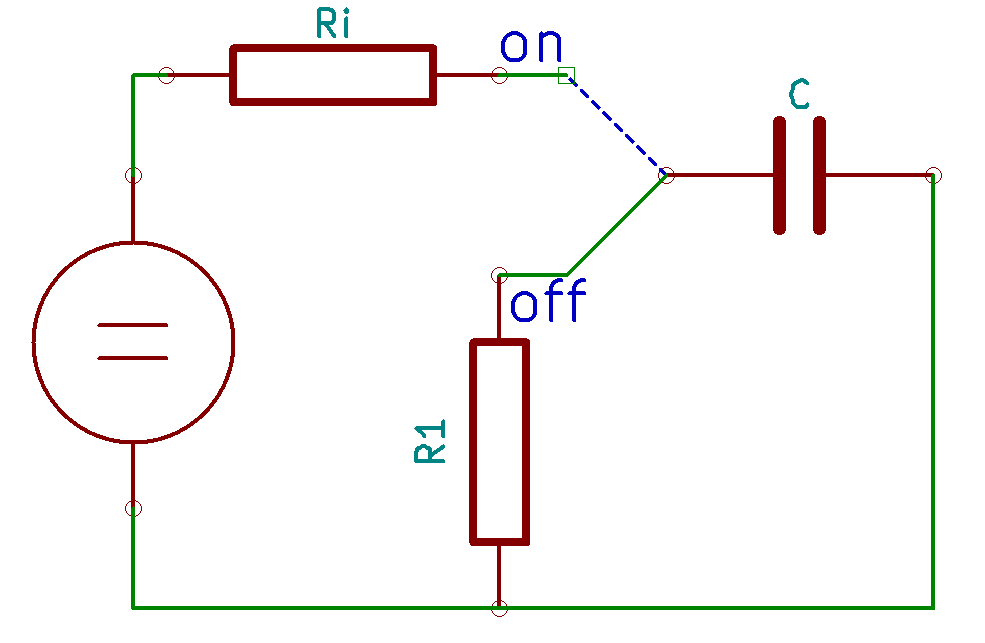
\includegraphics[width=0.5\textwidth]{Graphics/RC_circuit_discharge.png}
      \caption{RC-Schaltung, Kondensator entladen}{}
     \label{discharge_capacitor_circ}
\end{figure}

\noindent Auch beim Entladen eines Kondensators spielt die Zeitkonstante \(\tau \) eine wichtige Rolle. Der Entladevorgang ist nach \(5\tau \) abgeschlossen. Der während des Entladens fließende Strom lässt sich über das Ohmsche Gesetz 

\begin{equation}
  I_c = - \frac{U_c}{R_1}
  \label{eq:Ohm}
\end{equation}

\noindent ermitteln, sodass sich eine Entladekurve nach folgendem Beispiel ergibt.

\begin{figure}[H]
  \centering
      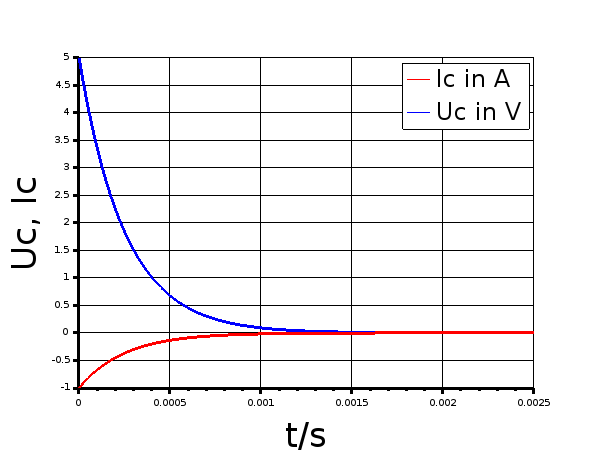
\includegraphics[width=\textwidth]{Graphics/KondensatorEntladekurve.png}
      \caption{R=5Ohm, C=50µF, Kondensator entladen}{}
     \label{discharge_capacitor}
\end{figure}

\clearpage
}
\endgroup}
%----------------------------------------------------------------------------------------

%----------------------------------------------------------------------------------------
%	Coil
%----------------------------------------------------------------------------------------
\newcommand*{\coil}{\begingroup
\subsection{Spule}\label{sec:coil}
{
\begin{figure}[H]
  \centering
      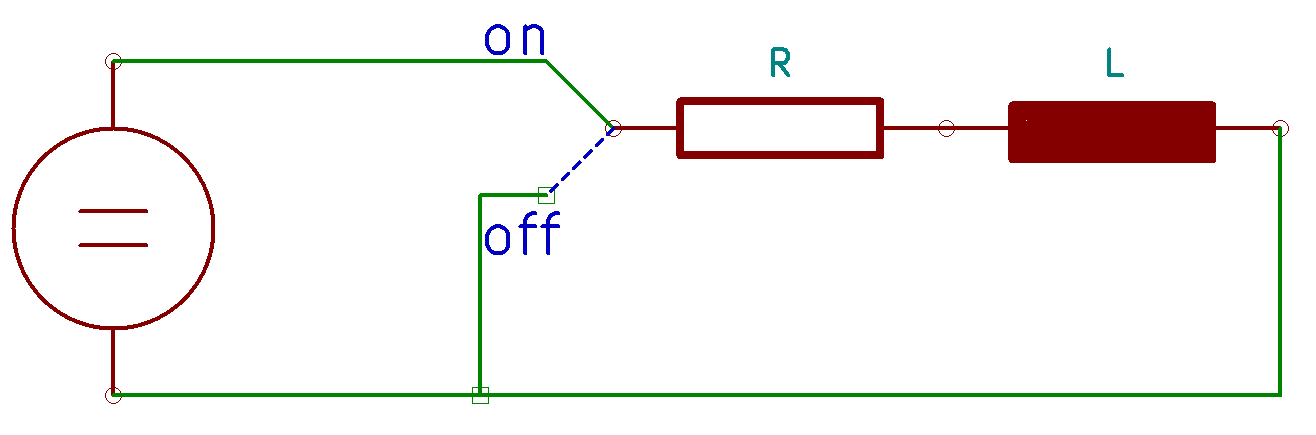
\includegraphics[width=0.75\textwidth]{Graphics/RL_circuit_on.png}
      \caption{RL-Schaltung, eingeschaltet}{}
     \label{coil_on}
\end{figure}

\noindent Wird eine Betriebsspannung \textbf{U} an eine Spule \textbf{L} angelegt (Abbildung \ref{coil_on}), so beginnt durch die Spule ein Strom \textbf{I} zu fließen, welcher ein magnetisches Feld erzeugt. Dieses magnetische Feld wiederum induziert in der Spule eine Spannung \(U_l\), welche der Betriebsspannung \textbf{U} entgegen wirkt. Diese selbstinduzierte Spannung beeinflusst den Stromfluss \(I_l\) nach folgender Gleichung.

\begin{equation}
  I_l = \frac{U - U_l}{R}
  \label{eq:currentCoil}
\end{equation}

\noindent Zum Zeitpunkt des Einschaltens (t=0) gilt

\begin{equation}
  U_l = U 
\end{equation}

\noindent sodass \(I_l = 0\). Man sagt auch \textbf{an einer Spule eilt der Strom der Spannung nach!} Für die Zeitkonstante \(\tau\) einer Spule gilt

\begin{equation}
  \tau_l = \frac{L}{R}
  \label{eq:tauCoil}
\end{equation}

\noindent Nach Ablauf eines \(\tau \) erreicht der Strom \(I_l\) in der Spule etwa 63\% des Gesamtstroms und nach \(5\tau \) erreicht dieser 99,3\%. Ab diesem Zeitpunkt wird der Einschaltvorgang in der Regel als abgeschlossen angesehen. Visuell dargestellt ergibt sich für den Einschaltvorgang einer Spule ein Diagramm nach folgendem Beispiel.

\clearpage

\begin{figure}[H]
  \centering
      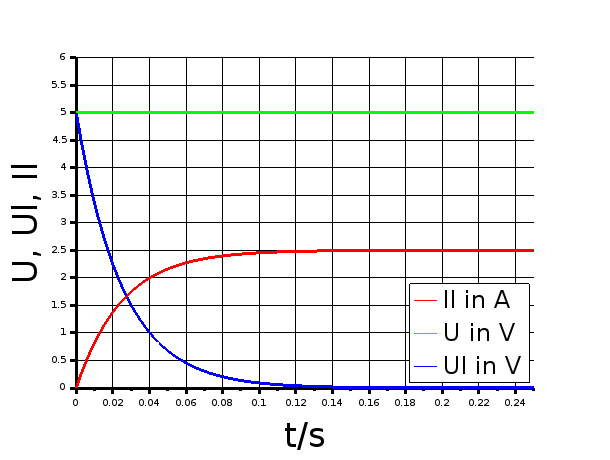
\includegraphics[width=\textwidth]{Graphics/SpuleLadekurve.png}
      \caption{U=5V, R=2hm, L=50mH, Einschaltvorgang einer Spule}{}
     \label{coil_on_diagram}
\end{figure}

\noindent Wird die Spannungsquelle abgeschaltet (Abbildung \ref{coil_off}) hält das magnetische Feld der Spule nach der Gleichung 

\begin{equation}
  W_l = \frac{1}{2} \cdot L \cdot I^2
  \label{eq:coilPower}
\end{equation}

\noindent eine Menge an Energie, welche eine Induktionsspannung \(U_l\) in Richtung der Betriebsspannung \textbf{U} erzeugt.

\begin{figure}[H]
  \centering
      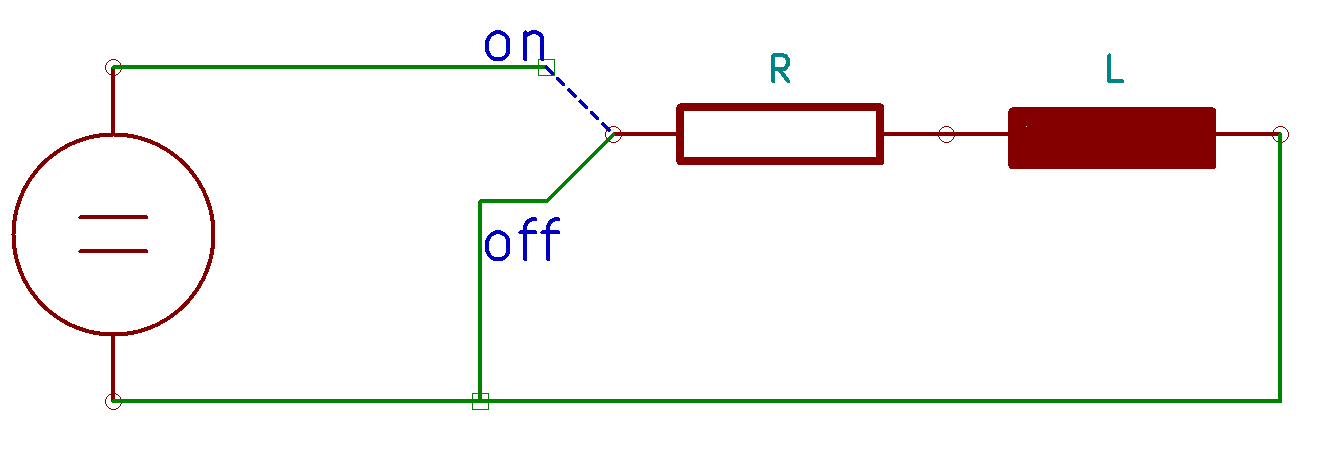
\includegraphics[width=0.75\textwidth]{Graphics/RL_circuit_off.png}
      \caption{RL-Schaltung, ausgeschaltet}{}
     \label{coil_off}
\end{figure}

\noindent Diese hält den Stromfluss auch nach Abschalten der Betriebsspannung \textbf{U} aufrecht, wodurch sich ein Diagramm nach folgendem Beispiel ergibt.

\begin{figure}[H]
  \centering
      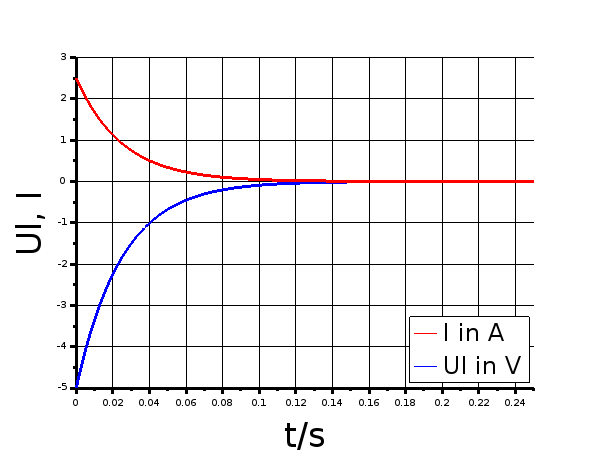
\includegraphics[width=0.95\textwidth]{Graphics/SpuleEntladekurve.png}
      \caption{U=0V, R=2hm, L=50mH, Abschaltvorgang einer Spule}{}
     \label{coil_off_diagram}
\end{figure}


}
\endgroup}
%----------------------------------------------------------------------------------------

%----------------------------------------------------------------------------------------
%	Serial Resonance circuit
%----------------------------------------------------------------------------------------
\newcommand*{\serialResonanceCircuit}{\begingroup
\section{Reihenresonanzkreis}\label{sec:serialresonancecircuit}
{\noindent 
\begin{wrapfigure}{r}{0.5\textwidth}
    \begin{minipage}[r]{0.5\textwidth}
      \vspace{-16pt}
\begin{figure}[H]
  \centering
  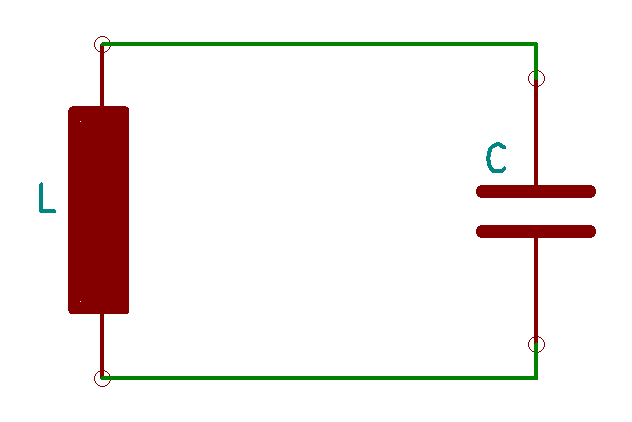
\includegraphics[width=\textwidth]{Graphics/ResonanceCircuit_simple.png}
  \caption{Idealer Resonanzkreis}{}
  \label{resonance_circuit_simple}
\end{figure}
      \vspace{-10pt}  
    \end{minipage}  
\end{wrapfigure}
\noindent Gegeben sei eine Schaltung bestehend aus einem geladenen Kondensator \textbf{C}, einer Spule \textbf{L} und frei von Widerständen. (Abbildung \ref{resonance_circuit_simple}) Der Kondensator entlädt sich über die Spule. Wie in Kapitel \ref{sec:coil} erläutert, wirkt die induzierte Spannung \(U_l\) der Betriebsspannung, also der Kondensatorspannung \(U_l\), entgegen. Nach \(5\tau \) ist sowohl der Einschaltvorgang der Spule abgeschlossen als auch der Kondensator komplett entladen. Da \(U_l = 0\) ist, hat der Strom seinen Maximum erreicht. Die im Magnetfeld der Spule gespeicherte Energie \(W_l\) treibt diesen Strom weiter und lädt den Kondensator in entgegengesetzter Richtung auf.

\clearpage

\begin{figure}[H]
  \centering
  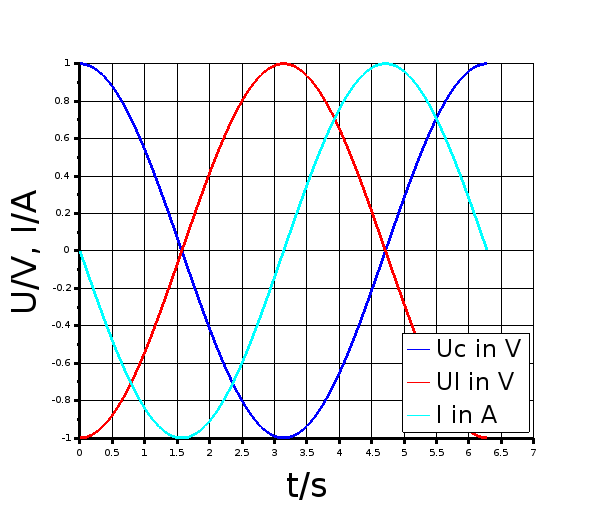
\includegraphics[width=\textwidth]{Graphics/ResonanceCircuit_UcUl.png}
  \caption{Spannungs- und Stromverlauf eines idealen Resonanzkreis}{}
  \label{resonance_circuit_simple_diagram}
\end{figure}

\noindent Ist \(W_l = 0\), entlädt sich der Kondensator wieder über die Spule. In Betrachtung der Annahme, diese Schaltung sei frei von Widerständen, schwingt die im System enthaltene Energie unendlich lange weiter und es ergibt sich ein Strom- und Spannungsverlauf wie in Abbildung \ref{resonance_circuit_simple_diagram} dargestellt\footnote{Stiny: Grundwissen Elektrotechnik, S. 287 f.}. Eine widerstandsfreie Schaltung ist in der Realität aber nicht möglich. Ein Wirkwiderstand R stellt die Summe aller reellen Widerstände der Schaltung dar. Dieser Widerstand hat zur Folge, dass die Schwingung gedämpft wird, also nach und nach abklingt. Das Beispiel soll nun um eine Wechselspannungsquelle \textbf{U} erweitert werden! (Abbildung \ref{resonance_circuit_serial})

\clearpage

\begin{wrapfigure}{r}{0.5\textwidth}
    \begin{minipage}[r]{0.5\textwidth}
      \vspace{-16pt}
\begin{figure}[H]
  \centering
  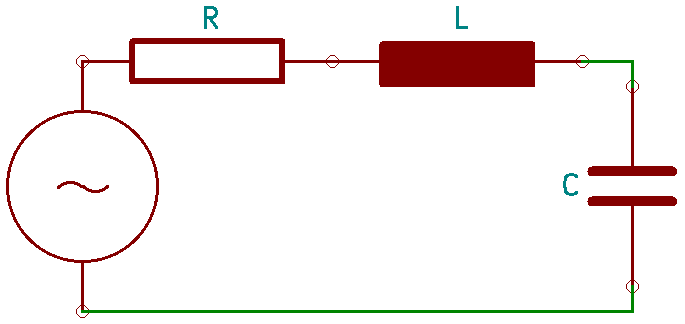
\includegraphics[width=\textwidth]{Graphics/ResonanceCircuit_serial.png}
  \caption{Reihenresonanzkreis}{}
  \label{resonance_circuit_serial}
\end{figure}
      \vspace{-10pt}  
    \end{minipage}  
\end{wrapfigure}

\noindent Die Spannungsquelle wirkt dem Abklingen der Schwingung entgegen indem Diese dem System mit der Frequenz \(f_0\) kontinuierlich neue Energie zuführt. Neben den reellen Widerständen beeinflussen Blindwiderstände die Schwingung. Zusammengefasst spricht man von der Impedanz \textbf{Z}. Diese wird als komplexe Zahl dargestellt, wobei die reellen Widerstände den Realteil und die Blindwiderstände den Imaginärteil darstellen.

\begin{equation}
  Z = R + j \cdot (\omega L - \frac{1}{\omega C})
  \label{eq:Impedance}
\end{equation}

\noindent Der daraus resultierende Scheinwiderstand lässt sich aus dem Betrag der Impedanz ermitteln.

\begin{equation}
  |Z| = \sqrt{R^2 + (\omega L - \frac{1}{\omega C})^2}
  \label{eq:Impedance2}
\end{equation}

\noindent Diese Gleichung zeigt deutlich, dass der Scheinwiderstand abhängig von der Dimensionierung des Kondensators \textbf{C} und der Spule \textbf{L} ist. Wählt man einen Kondensators \textbf{C} und eine Spule \textbf{L} so, dass gilt

\begin{equation}
  \omega L - \frac{1}{\omega C} = 0
  \label{eq:resonance}
\end{equation}

\noindent bedeutet dies für die Gleichung \eqref{eq:Impedance2}

\begin{equation}
  |Z| = \sqrt{R^2 + (0)^2} = \sqrt{R^2} = R
  \label{eq:ImpedanceResonance}
\end{equation}

\noindent Die Blindwiderstände heben sich gegenseitig auf, sodass der Scheinwiderstand ausschließlich aus dem Realteil besteht und somit als reell betrachtet werden kann. 

\begin{wrapfigure}{r}{0.5\textwidth}
    \begin{minipage}[r]{0.5\textwidth}
      \vspace{-16pt}
\begin{figure}[H]
  \centering
  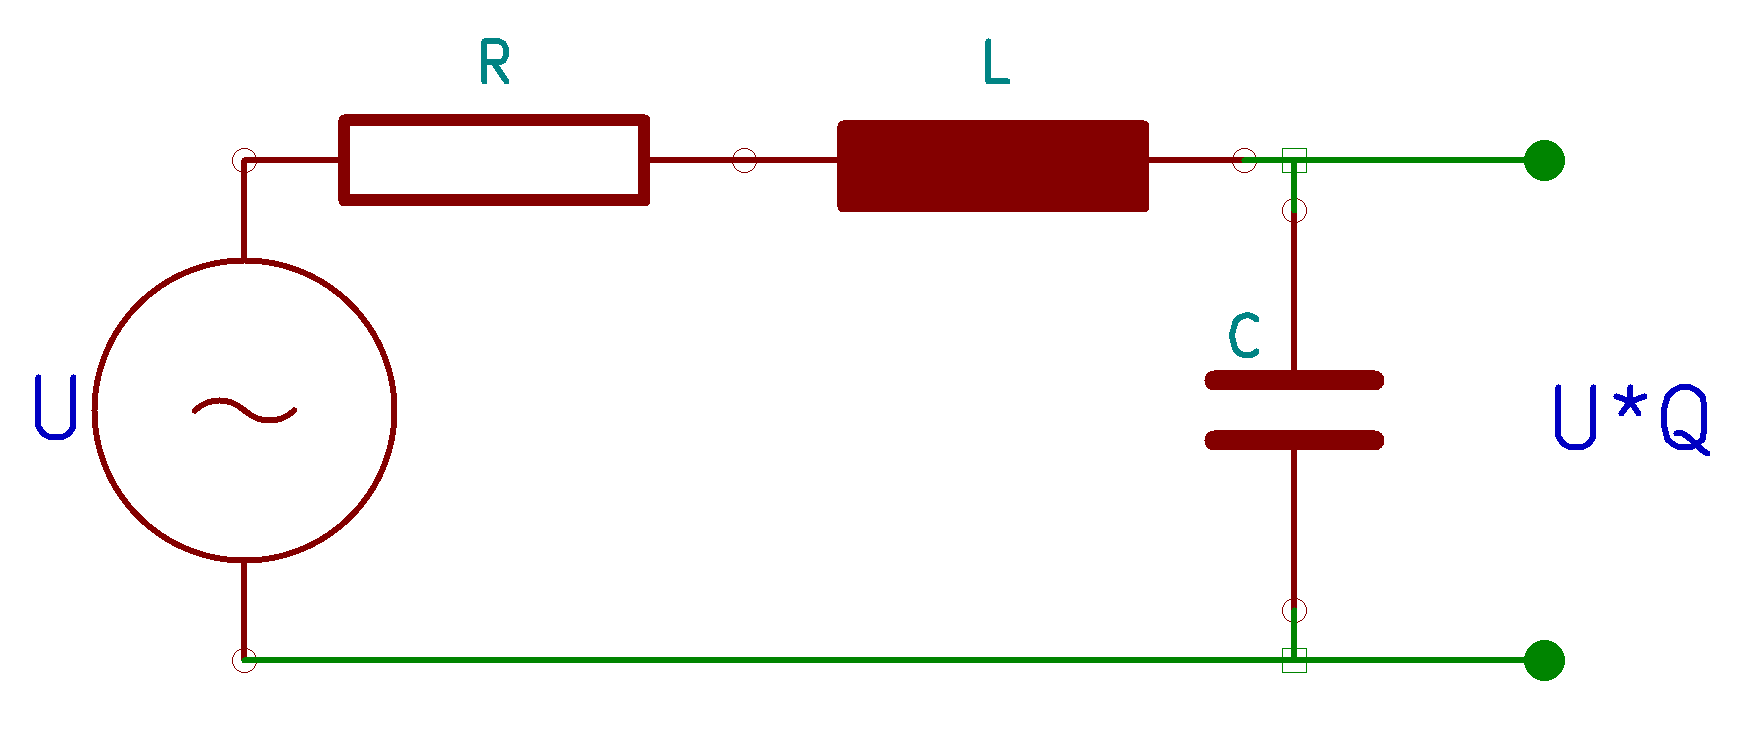
\includegraphics[width=\textwidth]{Graphics/ResonanceCircuit_quality.png}
  \caption{Resonanzkreis als Spannungsteiler}{}
  \label{resonance_circuit_quality}
\end{figure}
      \vspace{-10pt}  
    \end{minipage}  
\end{wrapfigure}

\noindent Wie Anfangs erwähnt weist der Reihenresonanzkreis die Eigenschaft auf, dass die Spannung an den Bauelementen abhängig von der Dimensionierung ist. Genauer gesagt kann die Spannung an der Spule und am Kondensator um ein Vielfaches höher sein als die Betriebsspannung \textbf{U}. Ausdrücken lässt sich dies über die Güte \textbf{Q} nach 

\begin{equation}
  Q = \frac{U_l}{U} = \frac{U_c}{U} = \frac{\omega L}{R} = \frac{1}{\omega RC} = \frac{1}{R} \cdot \sqrt{\frac{L}{C}}
  \label{eq:resonanceQuality}
\end{equation}

\noindent Je höher die Güte \textbf{Q}, desto höher ist die Spannung \(U_l\) und \(U_c\) im Verhältnis zur Betriebsspannung \textbf{U}. Um sich dies zu Nutze zu machen wird die Schaltung, durch das Abgreifen der Spannung parallel zum Kondensator, als Spannungsteiler genutzt. (Abbildung \ref{resonance_circuit_quality})
}
\endgroup}
%----------------------------------------------------------------------------------------
